\documentclass{article}
\newcommand{\rg}{\text{rg}}
% file's preambule
%%%%%%%%%%%%%%%%%%%



% connect packages
\usepackage[T2A]{fontenc}
\usepackage[utf8]{inputenc}
\usepackage[english]{babel}
\usepackage{hyperref}     % ТАК_НУЖНО
\hypersetup{unicode=true} % ТАК_НУЖНО
\usepackage{amsmath}
\usepackage{amssymb,textcomp, esvect,esint}
\usepackage{amsfonts}
\usepackage{amsthm}
\usepackage{graphicx}
\usepackage{indentfirst}
\usepackage{xcolor}
% \usepackage{enumitem} %--- ломал нумерацию!?

\usepackage{graphicx}
\usepackage{booktabs}
\usepackage{caption}
\usepackage{listings}
\usepackage{tikz}
\usepackage{xcolor}



\usepackage{media9}
\usepackage{animate}
\usepackage{threeparttable}
\usepackage{pifont}


\usepackage{import}
\usepackage{xifthen}
\usepackage{pdfpages}
\usepackage{transparent}

% \usepackage{natbib}

\usepackage[skip=1pt]{caption}

\usepackage{ifthen}
\definecolor{darkgreen}{RGB}{10,90,10}

% create environment

\newtheorem{to_thr}{Thr}[section]
\newtheorem{to_suj}[to_thr]{Suj}
\newtheorem{to_lem}[to_thr]{Lem}
\newtheorem{to_com}[to_thr]{Com}
\newtheorem{to_con}[to_thr]{Con}
\theoremstyle{definition}
\newtheorem{to_def}[to_thr]{Def}


\newenvironment{itemize*}
{
    \begin{itemize}
        \setlength{\itemsep}{1pt}
        \setlength{\parskip}{1pt}
        }
    {\end{itemize}
}

\newenvironment{enumerate*}
{
    \begin{enumerate}
        \setlength{\itemsep}{1pt}
        \setlength{\parskip}{1pt}}
    {\end{enumerate}
}

\newenvironment{description*}
{
    \begin{description}
        \setlength{\itemsep}{1pt}
        \setlength{\parskip}{1pt}}
    {\end{description}
}

\newmdenv[
  topline=false,
  bottomline=false,
  rightline=false,
  skipabove=\topsep,
  skipbelow=\topsep
]{leftrules}

% document palette

\definecolor{grey}{HTML}{666666}
\definecolor{ublue}{HTML}{08088A}
\definecolor{linkcolor}{HTML}{0000CC}
\definecolor{urlcolor}{HTML}{006600}
\hypersetup{
    pdfstartview=FitH,  
    linkcolor=linkcolor,
    urlcolor=urlcolor, 
    colorlinks=true,
    citecolor=blue}

% add (renew) commands
% базовая подстройка
\renewcommand{\d}{\, d}
\renewcommand{\leq}{\leqslant}
\renewcommand{\geq}{\geqslant}


% авторские команды
\newcommand{\vc}[1]{\mbox{\boldmath $#1$}}
\newcommand{\smallvc}[1]{\scalebox{0.65}{\mbox{\boldmath $#1$}}}
\newcommand{\T}{^{\text{T}}}
\newcommand{\con}{^{\dag}}
\newcommand{\sub}[2]{#1_{\textnormal{#2}}}
\newcommand{\vp}{\vphantom{\dfrac{1}{2}}}

% операторы (просто прямой текст)
\renewcommand{\Im}{\mathop{\mathrm{Im}}\nolimits}
\renewcommand{\Re}{\mathop{\mathrm{Re}}\nolimits}
% \renewcommand{\P}{\mathop{\mathrm{P}}\nolimits}
% \newcommand{\E}{\mathop{\mathrm{E}}\nolimits}
% \newcommand{\D}{\mathop{\mathrm{D}}\nolimits}
\newcommand{\cov}{\mathop{\mathrm{cov}}\nolimits}
\newcommand{\diag}{\mathop{\mathrm{diag}}\nolimits}
\newcommand{\card}{\mathop{\mathrm{card}}\nolimits}
\newcommand{\grad}{\mathop{\mathrm{grad}}\nolimits}
\renewcommand{\div}{\mathop{\mathrm{div}}\nolimits}
\newcommand{\rot}{\mathop{\mathrm{rot}}\nolimits}
\newcommand{\Ker}{\mathop{\mathrm{ker}}\nolimits}
\newcommand{\spec}{\mathop{\mathrm{spec}}\nolimits}
\newcommand{\sign}{\mathop{\mathrm{sign}}\nolimits}
\newcommand{\tr}{\mathop{\mathrm{tr}}\nolimits}
\newcommand{\rg}{\mathop{\mathrm{rg}}\nolimits}
\newcommand{\const}{\textnormal{const}}


% цветной текст
\newcommand{\red}[1]{\textcolor{red}{#1}}
\newcommand{\green}[1]{\textcolor{urlcolor}{#1}}
\newcommand{\blue}[1]{\textcolor{ublue}{#1}}


% символы
\newcommand{\cmark}{\text{\ding{51}}}
\newcommand{\xmark}{\text{\ding{55}}}


% подгрузка pdf_tex картинок
% \newcommand{\incfig}[1]{%
%     \def\svgwidth{\columnwidth}
%     \import{./figures/}{#1.pdf_tex}
% }


% специфично к квантам
\newcommand{\ket}[1]{\left| #1 \right\rangle}
\newcommand{\bra}[1]{\left\langle #1 \right|}

\newcommand{\dppp}{\frac{d^3 p}{(2 \pi \hbar)^3}}

\newcommand{\na}{$^{22}$Na}
\newcommand{\cs}{$^{137}$Cs}
\newcommand{\co}{$^{60}$Co}
\newcommand{\am}{$^{214}$Am}
\newcommand{\eu}{$^{152}$Eu}

% add page header
% add page header

\pagestyle{fancy}
\fancyhf{}
\fancyhead[RE,LO]{\textsc{Ф\raisebox{-1.5pt}{и}з\TeX}}
\fancyhead[LE,RO]{RQC}
\fancyhead[CO,CE]{\leftmark}
\fancyfoot[LE,RO]{\textcolor{grey}{\texttt{\thepage}}}



% matrixes shortcuts 
% \newcommand{\dmat}[4]{
  \ifthenelse{
    \equal{#1}{3}
  }{
\begin{pmatrix}
    #2 & 0 & 0 \\
    0 & #3 & 0 \\
    0 & 0 & #4 \\
\end{pmatrix}
  }{
  \ifthenelse{
      \equal{#1}{2}
    }{
  \begin{pmatrix}
      #2 & 0 \\
      0 & #3 \\
  \end{pmatrix}
    }{
      \text{\textcolor{red}{error}}
    }
  }
}

\newcommand{\skmat}[4]{
  \ifthenelse{
    \equal{#1}{3}
  }{
\begin{pmatrix}
    0 & -#4 & #3 \\
    #4 & 0 & -#2 \\
    -#3 & #2 & 0 \\
\end{pmatrix}
  }{
  \ifthenelse{
      \equal{#1}{2}
    }{
  \begin{pmatrix}
      0 & #2 \\
      -#2 & 0 \\
  \end{pmatrix}
    }{
      \text{\textcolor{red}{error}}
    }
  }
}

% additional symbols and commands


\DeclareRobustCommand{\tmpsim}{ %%%%%%%%%%%%%% ~ < %%%%%%%%%%%%%%%%%%%
  \mathbin{\text{
      \raisebox{-1pt}{
            \hspace{-4.5pt} \rotatebox{-26}{\scalebox{0.8}[0.7]{$\sim$}}
        }
  }}
}
\def\lesim{{
    \setbox0\hbox{$\ <\ $}
    \rlap{\hbox to \wd0{\hss$\tmpsim$\hss}}\box0
}}
%%%%%%%%%%%%%%%%%%%%%%%%%%%%%%%%%%%%%%%%%%%%%%%%%%%%%%%%%%%%%%%%%%%%%%


\def\letuscom{%%%%%%%%%%%%%%%%%%%%%% ПУСТЬ %%%%%%%%%%%%%%%%%%%%%%%%%%
\mathord{\setbox0=\hbox{$\exists$}%
     \hbox{\kern 0.125\wd0%
           \vbox to \ht0{%
              \hrule width 0.75\wd0%
              \vfill%
              \hrule width 0.75\wd0}%
           \vrule height \ht0%
           \kern 0.125\wd0}%
   }%
}
\newcommand{\letus}{\raisebox{-1.2pt}{$\letuscom$}}
%%%%%%%%%%%%%%%%%%%%%%%%%%%%%%%%%%%%%%%%%%%%%%%%%%%%%%%%%%%%%%%%%%%%%%


\usepackage{arydshln} %%%%%%%%%%%%%%% ЛИНИИ В МАТРИЧКЕ %%%%%%%%%%%%%%%
\makeatletter
  \renewcommand*\env@matrix[1][*\c@MaxMatrixCols c]{%
    \hskip -\arraycolsep
    \let\@ifnextchar\new@ifnextchar
  \array{#1}}
\makeatother
%%%%%%%%%%%%%%%%%%%%%%%%%%%%%%%%%%%%%%%%%%%%%%%%%%%%%%%%%%%%%%%%%%%%%%


\makeatletter %%%%%%%%%%%%%%% КРУЖОЧЕК %%%%%%%%%%%%%%%%%%%%%%%%%%%%%%%
\newcommand*{\encircled}[1]{\relax\ifmmode\mathpalette
\@encircled@math{#1}\else\@encircled{#1}\fi}
\newcommand*{\@encircled@math}[2]{\@encircled{$\m@th#1#2$}}
\newcommand*{\@encircled}[1]{%
  \tikz[baseline,anchor=base]{\node[draw,circle,outer sep=0pt,
                                        inner sep=.2ex] {#1};}}
\makeatother
%%%%%%%%%%%%%%%%%%%%%%%%%%%%%%%%%%%%%%%%%%%%%%%%%%%%%%%%%%%%%%%%%%%%%%











\usepackage{amssymb}
\usepackage{ mathrsfs }
\newcommand{\Lagr}{\mathcal{L}}
\newcommand{\R}{\mathbb{R}}
\begin{document}


\setlength{\abovedisplayskip}{3pt}
\setlength{\abovedisplayshortskip}{3pt}
\setlength{\belowdisplayskip}{3pt}
\setlength{\belowdisplayshortskip}{3pt}

% \numberwithin{equation}{section}

\begin{center}
    \LARGE \textsc{Задание по курсу <<Теория функций комплексного переменного I>>}
\end{center}

\hrule

\phantom{42}

\begin{flushright}
    \begin{tabular}{rr}
    % written by:
        \textbf{Автор}: 
        & Шишкин П.Е. \\ 
        &\\
    % date:f
        \textbf{От}: &
        \textit{\today}\\
    \end{tabular}
\end{flushright}

\thispagestyle{empty}
\tableofcontents 

\newpage
\section{I. Комплексные числа. Стереографическая проекция}

\subsection{\S1: 3(2)}
\subsubsection*{Условие}
\text {3. Найти все корни уравнения:}\\
2) $|z|-z=1+2 i$
\subsubsection*{Решение}
Положим $z=a + b i$
\begin{gather*}
    \sqrt{a^2 + b^2} - a - b i = 1 + 2i \\
    a^2 + b^2 = (1+ 2 i +a + b i )^2\\
    a^2+b^2 = a^2+2 i a b+(2+4 i) a-b^2-(4-2 i) b+(-3+4 i)\\
    2 (1 + a) (2 + b) i -3 + 2 a - 2 b (2 + b) = 0\\
    \begin{cases}
       (1+a)(2+b)=0\\
       -3 + 2 a - 2 b (2 + b) = 0\\
    \end{cases}\\
    \begin{cases}
      \left[
        \begin{gathered}
            a=-1\\
            b=-2\\
        \end{gathered}
        \right. \\
       -3 + 2 a - 2 b (2 + b) = 0
    \end{cases}\\
    \text{//тупой подстановкой каждого их вариантов получаем ответ//}\\
    \begin{cases}
        a=3/2\\
        b=-2\\
    \end{cases}
\end{gather*}
\subsubsection*{Ответ:}
$z=a+bi = 3/2 -2 i$

 \textcolor[rgb]{0.480469,0.566406,0.480469}{\textit{Вообще говоря можно было сразу заметить что b=-2 просто взглянув на мнимую часть слева и справа, но это слишком интеллектуально для меня}}                                               

\subsection{\S1: 4(2)}
\subsubsection*{Условие}
4. Решить систему уравнений:\\
2) $\left\{\begin{array}{l}\left|z^{2}-2 i\right|=4 \\ |z+1+i|=|z-1-i|\end{array}\right.$
\subsubsection*{Решение}
Поскольку геометрическое решение уже было разобрано, было бы скучно переписывать его (а ещё мне лень техать картинки). Заметим что $(1+i)^2 = 2i$ тогда получим:
\begin{gather*}
    \begin{cases}
        |z^2-(1+i)^2|=4\\
        |z+(1+i)|=|z-(1+i)|\\
    \end{cases}\\
    \begin{cases}
        |z+(1+i)|=|z-(1+i)|\\
        |z + (1 + i)| \cdot |z - (1+i)| = 2 \cdot 2
    \end{cases}\\
    \begin{cases}
        |z + (1 + i)| =2\\
         |z - (1+i)| = 2\\
    \end{cases}
\end{gather*}
Получается точка, удалённая на 2 от $1+i$ и от $-1-i$. 
\begin{figure}[h!]
\center{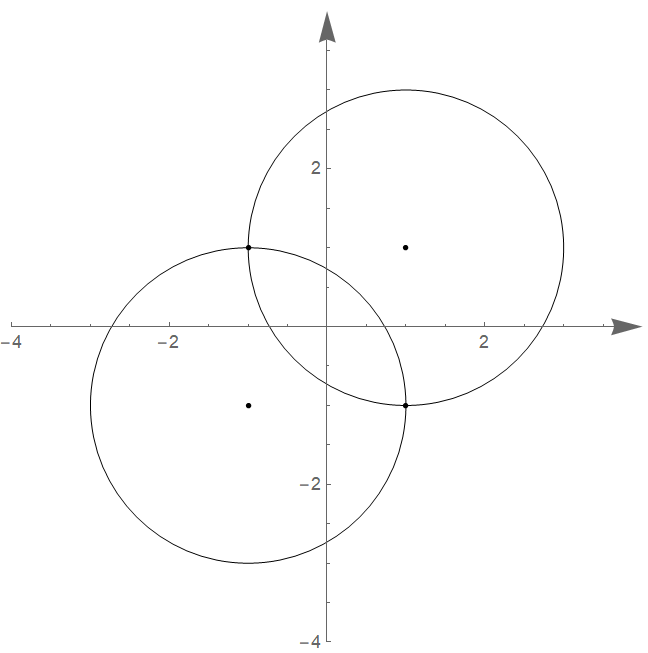
\includegraphics[width=0.8 \linewidth]{4(2).png}}
\caption{4(2)}
\label{fig:4(2)}
\end{figure} \\
Получается Ответом будут точки $z_1=-1+i; z_2 = 1-i$ это можно проверить также прямой подстановкой
\subsubsection*{Ответ:}
$z_1=-1+i; z_2 = 1-i$                       

\subsection{\S1: 11}
\subsubsection*{Условие}
11. Пусть $A$ и $C$ действительные, а $B$-комплексная постоянные и пусть $A C<|B|^{2} .$ Доказать, что уравнение
$$
A|z|^{2}+\bar{B} z+B \bar{z}+C=0 \quad(A>0)
$$
является уравнением окружности, а также найти центр этой окружности и ее радиус.
\subsubsection*{Решение}   
Пусть $\Re{z}=x; \Im{z}=y ; \Re{B}=b_1 ; \Im{B} = b_2$
\begin{gather*}
    A(x^2+y^2)+ (b_1- i b_2)(x+ iy)+(b_1+i b_2)(x-iy)+C=0\\
    A(x^2+y^2) + 2b_1 x+2b_2y+C=0\\
    (x^2+2 \frac{b_1}{A} x + \frac{b_1^2}{A^2})+ (y^2+2 \frac{b_2}{A} y + \frac{b_2^2}{A^2}) + C/A = \frac{b_1^2+b_2^2}{A^2}\\
    (x+b_1/A)^2+(y+b_2/A)^2 = \frac{|B|^2-AC}{A^2}
\end{gather*}
Ну уже очевидно - окружность с центром в точке $z_{cental}=-B/A$, радиусом $R=\frac{|B|^2-AC}{A^2}>0$
\subsubsection*{Ответ:}
 $z_{cental}=-B/A$, $R=\frac{|B|^2-AC}{A^2}>0$

\subsection{\S1: 18}
\subsubsection*{Условие}
18. Доказать, что три попарно различные точки $z_{1}, z_{2}, z_{3}$ лежат на одной прямой в том и только в том случае, когда величина $\frac{z_{3}-z_{1}}{z_{2}-z_{1}}$ действительна.
\subsubsection*{Решение}
Упростим данное условие домножив на сопряжённое:
\begin{gather*}
    \frac{(z_3-z_1)(\bar{z_2}-\bar{z_1})}{|z_2-z_1|^2} \in \R \\
    (z_3-z_1)(\bar{z_2}-\bar{z_1}) \in \R \\
    z_1 \bar{z_2} + \bar {z_1} z_3 - z_3 \bar z_2 \in \R\\
    (x_1+i y_1) (x_2 - i y_2) + (x_1-iy_1)(x_3+iy_3)-(x_3+iy_3)(x_2-iy_2) \in \R \\
    (x_3 (-y_1 + y_2) + x_2 (y_1 - y_3) + x_1 (-y_2 + y_3))i -x_2 x_3 + x_1 (x_2 + x_3) - y_2 y_3 + y_1 (y_2 + y_3) \in \R\\
    \text{//Что эквивалентно условию//}\\
    (x_3 (-y_1 + y_2) + x_2 (y_1 - y_3) + x_1 (-y_2 + y_3)) = 0\\
     \text{//немного преобразуя получаем//}\\
     (x_1 - x_2) (y_2 - y_3) - (y_1 - y_2) (x_2 - x_3)=0\\
     \text{//Это в свою очередь является z-компонентной произведения векторов//}\\
    \left( \begin{pmatrix}
         x1\\   
         y1\\
         0\\
     \end{pmatrix} - \begin{pmatrix}
         x2\\   
         y2\\
         0\\
     \end{pmatrix} \right) \times 
     \left( \begin{pmatrix}
         x2\\   
         y2\\
         0\\
     \end{pmatrix} - \begin{pmatrix}
         x3\\   
         y3\\
         0\\
     \end{pmatrix} \right) = 
     \begin{pmatrix}
         0\\   
         0\\
         (x_1 - x_2) (y_2 - y_3) - (y_1 - y_2) (x_2 - x_3)\\
     \end{pmatrix} = 
     \begin{pmatrix}
         0\\   
         0\\
         0\\
     \end{pmatrix}
\end{gather*}
Что собственно и доказывает требуемое в задаче утверждение. (вектор соединяющий одну пару точек коллинеарен вектору, соединяющему другую пару)
\subsubsection*{Ответ:}
Доказано

\subsection{\S2: 3}
\subsubsection*{Условие}
3. Пусть $\lim _{n \rightarrow \infty} z_{n}=A \neq \infty .$ Доказать, что
$$
\lim _{n \rightarrow \infty} \frac{z_{1}+z_{2}+\ldots+z_{n}}{n}=A
$$
\subsubsection*{Решение}
Если честно я не понимаю, в чём проблема рассмотреть отдельно действительную часть, отдельно мнимую. А потом сложить. Для действительных чисел уже доказывалось в курсе Математического анализа
\subsubsection*{Ответ:}
Я не понял условия

\subsection{T.1.}
\subsubsection*{Условие}
Т.1. Найти вещественную и мнимую части комплексных чисел:
a) $\left(\frac{1-i}{1+i}\right)^{2021}$
б) $(1+i)^{n}-(1-i)^{n}, n \in \mathbb{N}$
\subsubsection*{Решение}
а) \begin{gather*}
    \left(\frac{1-i}{1+i}\right)^{2021} = \left( \frac{\sqrt 2 \cdot \exp{(-\pi i /4)}}{\sqrt 2 \cdot \exp{(\pi i /4)}}\right)^{2021}=\\
    =\exp{(-\pi i /2)}^{2021} = \exp{(-\pi i /2 - 505 \cdot 2\pi i)} = \cos(-\pi/2) - i \sin(\pi/2) = -i
\end{gather*}     
б) \begin{gather*}
    (1+i)^{n}-(1-i)^{n} =\left (\sqrt 2 \right)^n (\exp{(\pi n i /4)} - \exp{(-\pi n i /4)}) = 2i \cdot 2^{n/2} (\sin{( \pi n /4)})
\end{gather*} 
\subsubsection*{Ответ:}
a) $-i$ b) $2i \cdot 2^{n/2} (\sin{( \pi n /4)}$
\subsection{T.2.}
\subsubsection*{Условие}
Т.2. Пусть $z_{1}, z_{2}, z_{3} \in \mathbb{C}$ не лежат на одной прямой. Найти выражение для центра окружности, проходящей через эти три точки.
\subsubsection*{Решение} 
\begin{gather*}
       \begin{cases}
           |z_1-z|=r\\
           |z_2-z|=r\\ 
           |z_3-z|=r\\
       \end{cases}
   \end{gather*}   
\subsubsection*{Ответ:}

\subsection{T.3.}
\subsubsection*{Условие}
Т.3. На единичной окружности $|z|=1$ взяты две точки $a$ и $b, a+b \neq 0$, и через них проведены касательные к окружности. Найти точку, в которой пересекаются эти касательные.
\subsubsection*{Решение}    
\subsubsection*{Ответ:}

\subsection{T.4.}
\subsubsection*{Условие}
Т.4. Покажите, что при стереографической проекции окружности на сфеpe Римана соответствует в комплексной плоскости окружность или прямая.
\subsubsection*{Решение}
\subsubsection*{Ответ:}

\subsection{T.5.}
\subsubsection*{Условие}
Т.5. Доказать, что для $z, z^{\prime} \in \mathbb{C}$ величина
$$
d\left(z, z^{\prime}\right)=\frac{2\left|z-z^{\prime}\right|}{\sqrt{\left(1+|z|^{2}\right)\left(1+\left|z^{\prime}\right|^{2}\right)}}
$$
выражает расстояние между прообразами этих точек при стереографической проекции.
\subsubsection*{Решение} 
\subsubsection*{Ответ:}

\subsection{T.6.}
\subsubsection*{Условие}
Т.6. Параметрическое уравнение прямой в комплексной плоскости можно записать в виде $z(t)=a+b t,-\infty<t<\infty$, где $a, b \in \mathbb{C}, b \neq 0 .$ При
этом направление прямой можно идентифицировать с направлением $b .$ Покажите, что неравенство $\operatorname{Im} \frac{z-a}{b}<0$ выделяет правую полуплоскость (относительно прямой), а неравенство Im $\frac{z-a}{b}>0$ выделяет левую полуплоскость.
\subsubsection*{Решение}
\subsubsection*{Ответ:}

\subsection{T.7.}
\subsubsection*{Условие}
Т.7. Пусть $a, b-$ ненулевые комплексные числа. Рассматривая их как векторы в комплексной плоскости, покажите, что $\operatorname{Re}\{\bar{a} b\}$-их скалярное произведение, а $|\operatorname{Im}\{\bar{a} b\}|$-площадь параллелограмма со сторонами $a$ и $b$.
\subsubsection*{Решение}  
\subsubsection*{Ответ:}

\subsection{T.8.}
\subsubsection*{Условие}
Т.8. Пусть $\omega_{0}, \omega_{1}, \omega_{2}, \ldots, \omega_{n-1},-$ корни $n$-ой степени из $1, n \geq 2 .$ Докажите, что выполняются следующие соотношения
$$
\sum_{k=0}^{n-1} \omega_{k}=0, \quad \prod_{k=0}^{n-1} \omega_{k}=(-1)^{n-1}
$$
\subsubsection*{Решение}
Заметим что множество ${\omega_i}$ совпадает с множеством решений уравнения $\omega^n + \omega^{n-1} \cdot 0 + ... + \omega \cdot 0 - 1=0$. Тогда применением теоремы Виета для коэффициентов при $\omega^{n-1}$ и при $\omega^0$ получим необходимые соотношения.
\begin{gather*}
    0= a_1 = \sum_{k=0}^{n-1} \omega_{k}\\
    1 = a_n = (-1)^n \prod_{k=0}^{n-1} \omega_{k}\\
\end{gather*}
Что и требовалось доказать
\subsubsection*{Ответ:}
Доказано.
\subsection{T.9*.}
\subsubsection*{Условие}
$\mathbf{T . 9}^{*} .$ Доказать, что точки $z_{1}, z_{2}, z_{3}$ являются вершинами равностороннего треугольника в том и только том случае, если выполняется условие $z_{1}^{2}+z_{2}^{2}+z_{3}^{2}=z_{1} z_{2}+z_{2} z_{3}+z_{3} z_{1}$
\subsubsection*{Решение} 
Двумя преобразованиями (смещение вдоль оси и поворот) можно перенести одновременно $z_1, z_2$ на ось действительных числел. При этом равносторонний треугольник (если он был таковым) останется равносторонним.  Тогда достаточно рассмотреть частный случай когда $z_1,z_2 \in \R $  
\begin{gather*}
                      
\end{gather*}                  
\subsubsection*{Ответ:}

\end{document}
